A penalty kick is the most isolated and the most decisive event in football. The ball is placed eleven metres from goal, one player takes the kick, one goalkeeper defends a mouth two hundred and forty four centimetres high and seven hundred and thirty two centimetres wide, and the ball reaches the goal line in roughly four tenths of a second. Human reaction time, measured from the visual stimulus to the beginning of a lateral dive, sits between two hundred and three hundred milliseconds for trained goalkeepers, which leaves almost no margin for a decision taken after the ball has been struck. Goalkeepers therefore do not react to the ball at all. They read the kicker, and they commit to a side before contact. Every coaching manual describes the same set of cues, namely the angle of the run up, the orientation of the hips at the moment the plant foot lands, the position of the shoulders, and the swing plane of the kicking leg. KickSense is built on the observation that these cues are precisely the quantities that a modern pose estimation library recovers automatically from ordinary video. If a coach can learn to read a skeleton, a model can be trained to read the same skeleton, and the reading can be made explicit, repeatable and measurable rather than intuitive.

The problem matters beyond the individual save. Penalty shootouts decide knockout football at every level, and the analytical support available to a goalkeeper is still remarkably thin. Professional clubs employ analysts who watch hours of footage manually and assemble dossiers on opposition penalty takers, a process that is expensive, slow and inherently subjective. Below the professional tier the support disappears entirely. A university side, an academy team or a school goalkeeper has no realistic path to a quantified profile of an opponent's penalty technique. The barrier is not the availability of video, because almost every match at every level is now recorded on a phone, but the availability of analysis. KickSense addresses exactly that gap by turning a single short clip, of the kind anyone can record from behind the goal or from the side of the pitch, into a structured prediction: the side the kicker is preparing to shoot towards, the confidence attached to that prediction, and an estimate of how firmly the ball is about to be struck. The system requires no motion capture suit, no calibrated multi camera rig and no wearable sensor, which is the property that makes it deployable in the environments where analytical support is currently absent.

The work completed so far establishes the full analytical chain end to end, and every component of that chain is operational rather than conceptual. A corpus of three hundred and one penalty kick videos was assembled from broadcast tournament footage and from sessions recorded specifically for this project, and two hundred and fifty nine of those clips carry a complete manual annotation covering shot direction, shot power, outcome, ball placement and the kicker's dominant foot. Each clip is decomposed into individual frames, each frame is passed through MediaPipe Pose to recover thirty three body landmarks with a visibility score, and the resulting variable length landmark stream is converted into a fixed size tensor of twenty six time steps by one hundred and thirty two features through hip centred translation, torso height scaling and linear temporal resampling. Two hundred and twenty five of the annotated clips survive the pose quality filters and form the modelling dataset, split into one hundred and fifty seven training, thirty four validation and thirty four test sequences with the class proportions preserved. A multi task network combining one dimensional convolutions with stacked Long Short Term Memory layers consumes these tensors and produces both a three way direction classification and a scalar power regression from a shared representation. The strongest configuration recorded a validation direction accuracy of 55.9 percent, well above the 33.3 percent expected from random guessing on three classes, and the pipeline is exposed through a Streamlit demonstration application that accepts an uploaded clip and returns the prediction with the pose overlay drawn on the video. The benefit of having built the chain in this order is that the expensive and irreversible part of the project, namely the collection and annotation of a bespoke dataset that does not exist publicly, is now complete and reusable. Every subsequent improvement, whether an architectural change, a hyperparameter search or an additional label, operates on the same stored intermediate artefacts and can be evaluated against the same held out split without repeating any of the earlier stages.

The limitations that motivated the project are the same ones that make the current results honest rather than impressive, and it is worth stating them plainly. Existing academic work on penalty prediction is almost entirely built on proprietary or unpublished datasets, which makes reproduction impossible and comparison meaningless. The approaches that report the strongest numbers depend on heavy machinery, typically semantic video segmentation followed by three dimensional convolution over full pixel volumes, which demands substantial computation and cannot run on a phone or on the modest hardware available to a non professional team. Broadcast footage, which is the only large scale source of penalty video, is filmed for entertainment rather than analysis, so camera angles change between clips, the kicker is frequently partially occluded by defenders or by the frame edge, resolution varies, and the moment of contact is often cut away to a crowd reaction. KickSense copes with these constraints deliberately rather than accidentally. Working on skeleton coordinates instead of pixels reduces each frame from hundreds of thousands of values to one hundred and thirty two, which shrinks the model to under a quarter of a million parameters and makes training feasible on a laptop and inference feasible in real time. Hip centred normalisation and torso height scaling remove the camera position and the apparent size of the player from the representation, so a clip filmed from behind the goal and a clip filmed from the touchline become comparable. Temporal resampling to a fixed twenty six steps removes the dependence on frame rate and clip length. An explicit quality gate rejects any clip in which fewer than ten frames or fewer than twenty percent of frames yield a usable pose, which converts the occlusion problem from a source of silent label noise into a measured and reported rejection rate. What remains, and what the remainder of this report does not attempt to hide, is that two hundred and twenty five sequences is a small dataset for a temporal deep learning model, that the class distribution is uneven, that the power annotation is a subjective human judgement rather than a physical measurement, and that the resulting accuracy is meaningfully better than chance but not yet at a level that would be trusted in a competitive setting.

\begin{figure}[H]
    \centering
    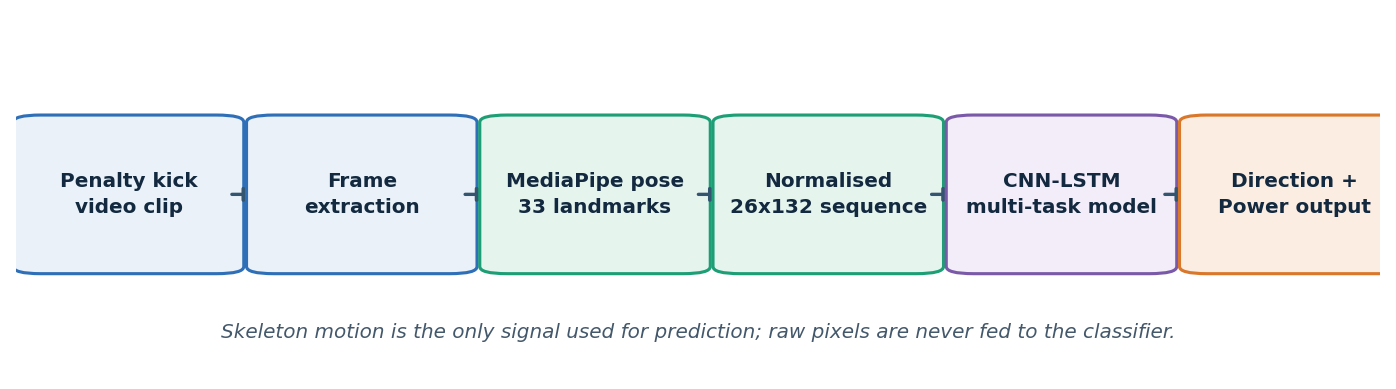
\includegraphics[width=0.99\textwidth]{fig01_concept_overview.png}
    \caption{Conceptual overview of the KickSense processing chain}
    \label{fig:concept}
\end{figure}

\noindent
\textbf{Description:} This figure states the method in its shortest form. A penalty clip is decomposed into frames, each frame is reduced to a thirty three landmark skeleton, the skeleton stream is normalised and resampled into a fixed size tensor, and a multi task network predicts both the shot direction and the shot power from that tensor. The property that defines the approach is that raw pixels never reach the classifier, so the model cannot learn from kit colour, stadium, crowd or broadcast graphics, only from how the kicker moves.

\section{Background}

Football analytics has moved through three broad phases. The first was notational analysis, in which trained observers manually tallied events such as passes, shots and tackles from video, producing reliable but extremely labour intensive data. The second was automated event and trajectory tracking, in which optical systems installed in stadiums recovered the positions of all players and the ball at high frequency, enabling spatial and tactical analysis at scale but requiring infrastructure available only to elite competitions. The third and current phase is the analysis of individual technique, in which the interest shifts from where a player is to how a player moves, and this is the phase in which human pose estimation has become the enabling technology.

Human pose estimation recovers the two dimensional or three dimensional coordinates of anatomical keypoints from an image. The field advanced rapidly after the introduction of convolutional architectures that predict per joint heatmaps, and it became practically deployable when lightweight pipelines began to run at interactive frame rates on commodity hardware. MediaPipe Pose, the library used in this project, follows a two stage detector and tracker design and returns thirty three landmarks per frame, each with a normalised horizontal coordinate, a normalised vertical coordinate, a depth estimate relative to the hip midpoint, and a visibility confidence. The significance for sports analysis is that a video sequence can be reduced to a compact numerical description of body motion, discarding kit colour, pitch texture, crowd background and broadcast graphics while retaining the biomechanical content that actually determines the outcome of a technical action.

The specific biomechanics of penalty kicking have been studied extensively in sports science, and the findings are consistent. The orientation of the pelvis at the instant the support foot is planted is the single strongest predictor of shot direction, because the hips must open towards the target for the leg to swing through the ball on the required line. The angle of the run up approach, the lean of the trunk, the position of the non kicking arm used for balance, and the height and speed of the backlift of the kicking leg all carry additional directional information. Shot power correlates with the angular velocity of the shank at contact, with the length of the backswing, and with the forward momentum generated during the final approach stride. Each of these quantities is, at least in principle, recoverable from the landmark trajectories that MediaPipe produces, which is what makes a pose driven model a natural fit for this task rather than an arbitrary architectural choice.

The remaining background element is the state of publicly available data. There is no standard benchmark dataset for penalty kick direction prediction. General purpose action recognition corpora contain football clips but do not annotate penalty direction or power. Sports specific datasets tend to focus on event spotting, player detection or tracking rather than on the fine grained technique of a single isolated action. This absence is the reason a bespoke corpus had to be collected and annotated for this project, and it is also the reason that a direct numerical comparison against published penalty prediction results cannot be made fairly, a point developed further in Chapter 2 and quantified in Chapter 4.

\section{Objective}

The objective of KickSense is to demonstrate that the directional and power intent of a football penalty kick can be predicted from the kicker's body motion alone, using only ordinary single camera video, at a computational cost low enough for the system to run on consumer hardware. The prediction must be produced before the moment of ball contact is required as input, so that the output is genuinely anticipatory rather than a retrospective description of a completed event, and it must be accompanied by a calibrated confidence value so that a user can distinguish a confident reading from an uncertain one.

Supporting this primary objective is a methodological aim of equal importance to the project, namely that every stage of the pipeline should be reproducible and independently inspectable. Intermediate artefacts are written to disk at every step, so extracted frames, landmark arrays, normalised tensors and the stratified split indices all persist between runs. This makes it possible to change one component, retrain, and attribute the resulting difference in accuracy to that component alone, which is the property that the ablation study reported in Chapter 4 depends on.

\section{Problem Description}

The core problem is a temporal sequence classification problem under severe data scarcity and severe input variability. Given a short video clip of a football penalty kick, the system must assign the clip to one of three directional classes and produce a scalar power estimate, using a training set of a few hundred examples drawn from footage that was never intended for analytical use. Several distinct difficulties combine to make this hard, and each was observed directly during development rather than anticipated from the literature.

\begin{enumerate}[label=\roman*.]
    \item Broadcast penalty footage is filmed from inconsistent camera positions, so the same physical motion produces very different pixel patterns and very different raw landmark coordinates across clips.
    \item The kicker is frequently occluded by the goalkeeper, by teammates in the frame, or by the edge of the frame itself, which causes MediaPipe to fail on a substantial fraction of frames.
    \item Clip lengths and frame rates vary widely, so the number of frames available per kick ranges from a few dozen to several hundred and cannot be assumed constant.
    \item The three directional classes are not balanced, because penalty takers in real matches shoot to the corners far more often than down the middle.
    \item Shot power has no ground truth measurement available from video, so the annotation is a human judgement on a one to ten scale and carries irreducible subjective noise.
    \item The total quantity of labelled data is small relative to the capacity of any temporal deep learning architecture, which makes overfitting the default outcome unless it is actively suppressed.
\end{enumerate}

\section{Project Objectives}

The project was decomposed into a set of concrete, verifiable objectives, each of which maps onto a specific deliverable in the codebase.

The first objective is the construction of an annotated penalty kick corpus, since no suitable public dataset exists. This required sourcing broadcast clips across multiple tournaments, recording additional footage locally to increase the volume and the diversity of camera angles, cutting each source video down to the penalty action itself, and manually annotating shot direction, shot power, outcome, ball placement, dominant foot, match and tournament for every clip in a single spreadsheet that acts as the project's label authority.

The second objective is a reliable pose extraction stage that converts video into landmark sequences and reports its own failure rate honestly. This means running MediaPipe Pose at its highest model complexity over every extracted frame, storing the resulting landmark array per clip, and recording how many frames yielded a detection so that clips with insufficient pose coverage can be identified and excluded rather than silently degrading the training signal.

The third objective is a preprocessing stage that makes clips comparable to one another. Raw landmark coordinates are dominated by where the player happens to stand in the frame and how large the player appears, neither of which carries any information about shot direction. The preprocessing stage removes both effects through hip centred translation and torso height scaling, and removes the effect of variable clip duration through resampling to a fixed number of time steps.

The fourth objective is a multi task predictive model that produces both outputs from a shared representation, on the reasoning that the body motion which determines direction also determines power, so a shared encoder should be more sample efficient than two independent models trained on the same small dataset.

The fifth objective is an honest evaluation protocol. The system must be assessed on a held out test split that is never used for model selection, using accuracy, per class precision, recall and F1 score, a confusion matrix, and regression error metrics for the power head, with the three class random baseline stated explicitly so that any reported accuracy can be interpreted correctly.

The sixth objective is a usable interface. A Streamlit application accepts an uploaded clip, runs the full pipeline, renders the pose overlay so that the user can see what the model actually observed, and displays the direction prediction with its confidence distribution alongside the power estimate. A FastAPI service wraps the same inference path so that the planned mobile and web client can call it over HTTP.

\section{Project Scope}

The scope of the current phase of KickSense covers the complete offline analytical pipeline together with a single user demonstration interface. In scope are dataset collection and annotation, frame extraction, pose estimation, preprocessing and normalisation, model construction, training with augmentation and regularisation, quantitative evaluation on a held out split, ablation analysis of the architectural and training choices, qualitative inspection of pose overlays, and the Streamlit demonstration application together with the FastAPI wrapper that exposes the inference path as a service.

Deliberately outside the scope of this phase are several capabilities that would be natural extensions but that were not attempted, and it is important to be explicit about them rather than imply a completeness the system does not have. The system does not track the ball, so the ball placement annotation present in the label file is recorded but unused by the model. The system does not perform goalkeeper analysis, so it makes no recommendation about where a keeper should dive and no assessment of the keeper's own movement. The system operates on a single kicker per clip and does not handle multi player scenes. It does not run on video streams in real time from a camera feed, only on uploaded files. It produces no three dimensional reconstruction of the kick, since the depth value returned by MediaPipe is a relative estimate rather than a calibrated measurement and was not found to be reliable enough to build on. Finally, the mobile client is designed but not implemented, which is why it appears in the future work of Chapter 5 rather than in the results of Chapter 4.

\section{Solution Application Areas}

The most direct application is goalkeeper preparation. A goalkeeper or goalkeeping coach can assemble clips of an opponent's previous penalties and obtain a quantified profile of that player's directional tendencies together with the confidence of each reading, which converts an informal impression into something that can be reviewed, argued with and updated as new footage arrives.

A second application is technique coaching for the kicker rather than the keeper. If a model can identify the side a kicker is aiming for from the body motion alone, then that kicker's motion is leaking their intention, and the specific landmark trajectories that drove the prediction indicate where the leak is. A player whose direction is predicted with high confidence from the hip orientation at plant foot contact has a concrete, actionable technical flaw to work on.

A third application is academic and pedagogical. The pipeline is a compact, fully documented example of skeleton based temporal action analysis on a real and difficult dataset, and the intermediate artefacts at every stage make it suitable as a teaching resource for computer vision and sequence modelling. The honest reporting of the failure modes, in particular the pose detection failure rate on broadcast footage and the impact of a small unbalanced dataset, is arguably more instructive than a polished result would be.

A fourth application area, contingent on the mobile client planned in Chapter 5, is grassroots and academy use. The defining property of the system is that it requires only a phone camera and no installed infrastructure, so the analytical support currently confined to professional clubs becomes accessible to teams that have video but no analysts.

\begin{figure}[H]
    \centering
    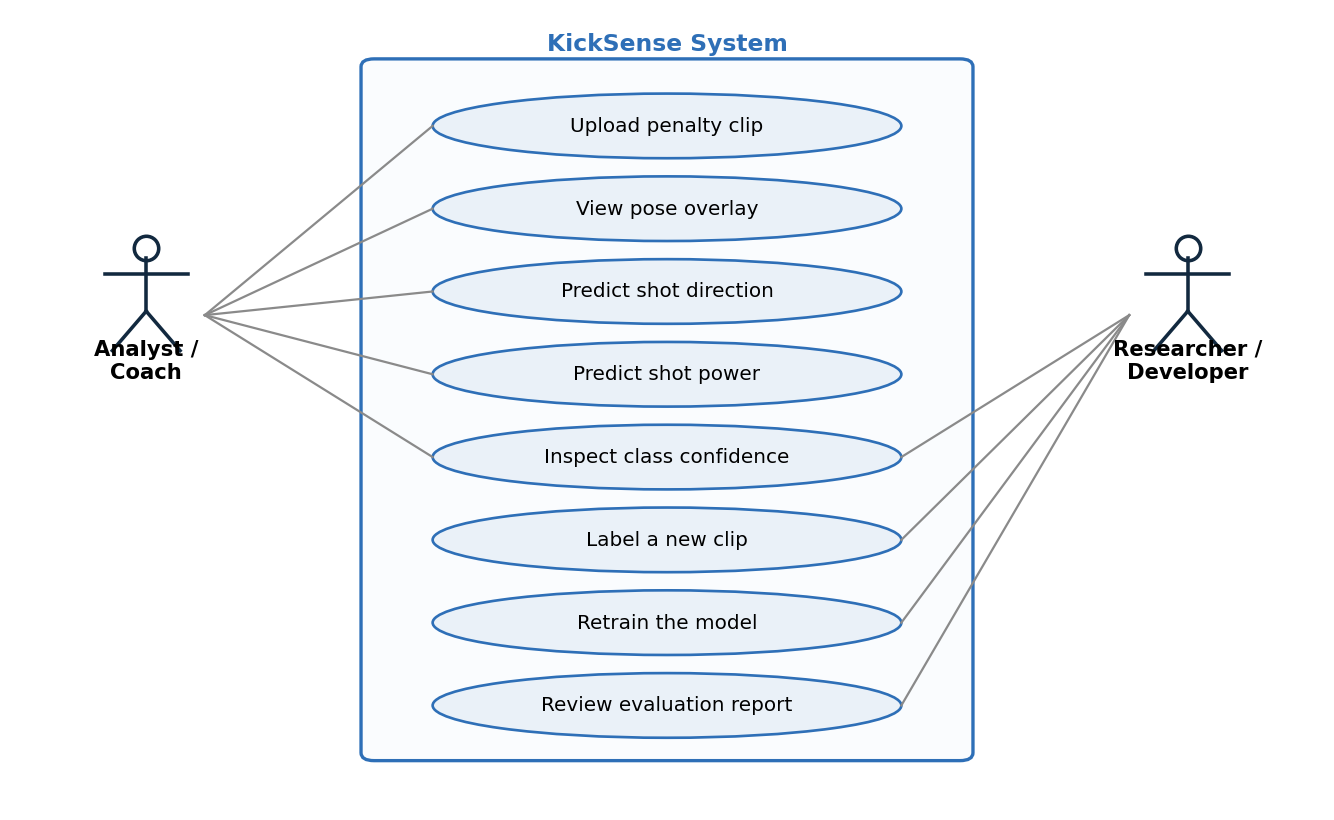
\includegraphics[width=0.95\textwidth]{fig03_usecase_diagram.png}
    \caption{Use case diagram of the KickSense system}
    \label{fig:usecase}
\end{figure}

\noindent
\textbf{Description:} This diagram identifies the two actors the system serves and the operations available to each. The analyst or coach uploads a penalty clip, inspects the rendered pose overlay to confirm the system observed the player correctly, and reads the direction and power predictions together with the class confidence distribution. The researcher or developer additionally annotates new clips, retrains the model on the expanded corpus, and reviews the evaluation report. Inspecting class confidence is available to both actors, because a prediction accompanied by a low confidence value should be treated differently from a confident one by anyone reading it.

\section{Risk Involved}

\subsection{Data Scarcity and Class Imbalance}

The most significant risk to the project is the size of the dataset. Two hundred and twenty five usable sequences is small for a model containing roughly a quarter of a million parameters, and the direction classes are unbalanced with one hundred and seven left, ninety four right and fifty eight centre examples. The consequences are visible in the results, since the model overfits the training set rapidly and the centre class is recognised least reliably. The risk is mitigated but not eliminated by a fivefold augmentation strategy, by aggressive dropout and batch normalisation, by early stopping on validation accuracy, and by a stratified split that guarantees every class appears in every partition. The residual risk is managed by continuing to record additional footage, with the locally recorded sessions already contributing sixty one clips to the corpus.

\subsection{Pose Estimation Failure on Broadcast Footage}

The pipeline is entirely dependent on MediaPipe recovering a usable skeleton, and on broadcast footage this frequently fails because the kicker is occluded, small in frame, or motion blurred. If failures were allowed through silently they would inject sequences of interpolated or duplicated frames into the training data and corrupt the learned representation. The mitigation is the explicit quality gate described in Chapter 3, which rejects clips falling below a minimum absolute frame count and a minimum detection ratio, and which converts a hidden data quality problem into a reported and quantified rejection rate. The cost of this mitigation is a smaller dataset, which feeds directly back into the first risk.

\subsection{Label Subjectivity in the Power Annotation}

Shot direction is objectively verifiable from the footage, but shot power was annotated by human judgement on a one to ten scale with no instrumented ground truth. The distribution of these labels is heavily concentrated, with a large cluster at the maximum value, which suggests that the annotation compresses a continuous physical quantity into a coarse and inconsistently applied ordinal scale. The regression head therefore learns a target that is itself noisy, and its reported error should be read as an upper bound on achievable accuracy rather than as a measure of the model's capability. The mitigation applied is to weight the power loss at 0.3 relative to the direction loss so that noisy power targets cannot dominate the shared representation, and the planned mitigation is to replace the subjective scale with a measurement derived from ball displacement between consecutive frames.

\subsection{Configuration Drift Between Training and Inference}

A practical engineering risk identified during development is that the preprocessing applied at inference time must match the preprocessing applied at training time exactly, since any discrepancy silently degrades accuracy without producing an error. One such discrepancy was found in the pose estimation configuration, where the training pipeline and the interactive application did not use identical settings. The mitigation is that all preprocessing constants are defined in a single module which both paths import, and that the correction of the remaining configuration mismatch is listed as an explicit item in the future work of Chapter 5.

\clearpage
